\documentclass[a4paper, 11pt]{article}
\usepackage{graphicx}
\usepackage[a4paper,bindingoffset=0in,%
            left=1in,right=1in,top=1in,bottom=1in,%
            footskip=.25in]{geometry}
\usepackage[square,numbers]{natbib}

\begin{document}

\title{A Software Package for Extensible Decision Trees in C++}

\begin{titlepage}
	\centering
	\vspace{1cm}
	{\scshape\LARGE Ludwig-Maximilians-Universität München \par}
	\vspace{1.5cm}
	
\includegraphics[width=0.35\textwidth]{figure/lmu_logo.png}\par\vspace{1cm}
	\vspace{0.5cm}
	{\scshape\Large Bachelor Thesis in Computer Science\par}
	\vspace{1.5cm}
	{\huge\bfseries treelib - A Software Package for Extensible Decision Trees in C++\par}
	\vspace{2cm}
	{\Large\itshape Christian Alexander Scholbeck\par}
	\vfill
	supervised by\par
	Prof. Dr. Bernd Bischl \par
	Prof. Dr. Marvin Wright \par
	Dr. Giuseppe Casalicchio

	\vfill

% Bottom of the page
	{\large Month Day, 2021 \par}
\end{titlepage}

\newpage
\thispagestyle{empty}

\vspace*{4cm}
\begin{abstract}
This thesis provides a software package for extensible decision trees written in C++. The package follows object-oriented and modular design principles. It works as a standalone application, or can be called by other programming languages. It supports both binary and multiway splitting, and can be extended with new optimizing algorithms, split criteria, models, and objectives. Supported application areas include classic predictive modeling with decision trees such as CART or C4.5, and advanced modeling such as model-based recursive partitioning. Furthermore, the modular design principle allows the extension of the package to support novel applications such as surrogate modeling for interpretable machine learning.

\end{abstract}
\vspace{2cm}
\tableofcontents
\clearpage
\setcounter{page}{1}
\section{Introduction}

Decision trees are one of the most fundamental techniques in machine learning. They are frequently preferred over more complex models due to their intelligibility in the form of decision rules, e.g., in medical applications \cite{podgorelec_trees_medicine}. A decision tree recursively partitions the data and fits a model inside each partition. Tree learning algorithms are numerous and differ regarding split criteria, model choices and pruning \cite{loh_trees_review}.
\par
%Their most critical drawback is a high variance under perturbations of the training data \cite{hastie_elemstatlearn}. This has led to the development of tree ensembles such as random forests \cite{breiman_randomforests}, which reduce variance to the detriment of losing interpretability.

%such as CART minimize the sum of squared deviations from the mean target value for regression tasks, or Gini impurity for classification tasks. More complex variants such as MOB train predictive models inside the leaf nodes, e.g., (generalized) linear models. Most decision tree variants such as CART or MOB are restricted to binary splits, whereas others such as C4.5 enable multiway splitting, which increases computational complexity.
%\par
%The possibilities of applying decision trees in contexts other than such as interpretable machine learning are numerous. For instance, due to their intelligibility, decision trees are especially suited as a surrogate model for black box models, where the black box predictions are approximated by interpretable functions inside the leaf nodes.
\par
Applications for decision trees are numerous, e.g., predictive modeling, surrogate modeling, or density estimation. This creates a requirement for an accessible, efficient, and extensible software implementation of decision trees. Accessible, to benefit a broad scientific community. Efficient, as the computational demand of optimizing splits grows considerably with the tree's complexity. Extensible, as different applications require entirely different decision tree setups.
\par

\subsection{Contributions} The central contribution of this thesis is a from-the-ground-up implementation of extensible decision trees as an open-source software package. The package is written in \texttt{C++} to achieve a high degree of computational efficiency, while preserving object-oriented principles and portability to other programming languages. The package follows modular design principles to achieve a maximum degree of extensibility.
\par
The written thesis provides a compact literature review of decision trees and smart splitting. Furthermore, it describes the software design and extensibility to support other applications, and demonstrates the package on simulated and real data.

\subsection{Software Description}

The software can be run as a standalone application, and supports console outputs of tree information such as the tree structure, and node summaries. Furthermore, it can be called by other programming languages for the usage in more flexible application environments. The program specifications are determined at runtime. It supports an arbitrary number of splits. 
The modular structure allows the extension with 
new optimizing algorithms, split criteria, node models, and objectives. 

\section{Theory}

Decision tree learning algorithms recursively partition the data by optimizing an objective in a greedy way. Subsequent partitionings can be visualized as a series of decision rules, which together form a tree graph (see Fig. \ref{fig:tree_structure}). Each partitioning of the data is referred to as a node, whereas a final partitioning is referred to as a leaf node. The starting point of a decision tree, which encompasses the entire, unpartitioned data, corresponds to the root node.
\par
A predictive model is trained inside each node.
The decision tree predicts by sending an observation through the tree from the root node to a leaf node, and using the leaf node model to predict.
Decision trees are referred to as regression trees if the target is numeric, and classification trees, if the target is categorical.
\par
A critical drawback of decision trees is a high variance under perturbations of the training data \cite{hastie_elemstatlearn}. This has led to the development of tree ensembles such as random forests \cite{breiman_randomforests}, which reduce variance to the detriment of losing interpretability. The focus of this thesis and the software package lies on single decision trees.


\begin{figure}
    \centering
    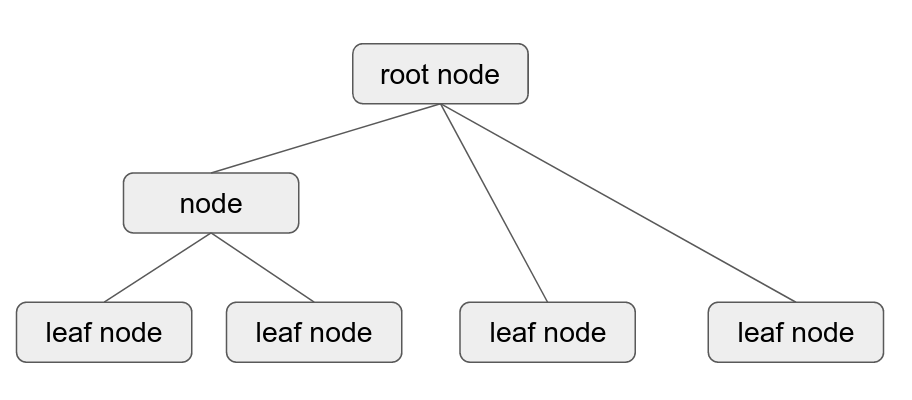
\includegraphics[width = 0.5 \linewidth]{thesis/figure/tree_structure.png}
    \caption{General decision tree structure comprising a root node, regular nodes, and leaf nodes.}
    \label{fig:tree_structure}
\end{figure}

\subsection{General Setup}

Each decision tree has five common components:
\begin{enumerate}
    \item \textbf{Node model choice:} What types of models are trained inside each node?
    \item \textbf{Objective function:} What objective function is to be optimized to find the best split?
    \item \textbf{Optimization:} How are possible split points generated to be tested for improvements?
    \item \textbf{Stopping:} When do we stop splitting?
    \item \textbf{Pruning:} How is the tree pruned post-hoc to avoid overfitting?
\end{enumerate}

\subsection{Variants}

An encompassing review of various decision tree variants is provided in \cite{loh_trees_review}. 
Classification and regression trees (CART) \cite{cart_1, cart_2, cart_3} and C4.5 \cite{quinlan_c45} are commonly used ones \cite{hastie_elemstatlearn} and date back several decades. Recent developments include conditional inference trees (CTREE) \cite{hothorn_ctree} and model-based recursive partitioning (MOB) \cite{zeileis_mob}.

\subsubsection{CART}

CART is restricted to binary splits.
For regression trees, CART fits a constant inside each node. The objective corresponds to the weighted sum of child node squared deviations from the fitted constant. The constant that minimizes the objective is the mean target value inside the node.
For classification trees, Gini impurity is minimized, which is based on the relative probabilities of the target classes inside the node. This spares the need for fitting a model, except for the leaf nodes, where CART uses a majority class vote. 
\par
The tree is fully grown until a pre-specified minimum node size criterion would be violated when splitting further. The tree height is pruned post-hoc according to a complexity parameter to avoid overfitting. The complexity parameter is estimated via cross-validation \cite{hastie_elemstatlearn}.

\subsubsection{C4.5}

C4.5 is restricted to classification trees. It uses an information-theoretic measure of node impurity based on entropy called gain ratio. C4.5  



\subsection{Smart Splitting}


\section{Related Work}

An initial software implementation of MOB was published as part of the \texttt{party} package \cite{party_package} for the \texttt{R} programming languge for statistical computing \cite{r_citation}. A more flexible version, which supports more inference options and is extensible to new models, was introduced in the \texttt{partykit} package \cite{partykit_package}. 
\par
The \texttt{R} language is able to directly call \texttt{C} or \texttt{C++} code, which warrants significant speedups in computational execution time \cite{eddelbuettel_rcpp}. However, software implementations which are solely written in \texttt{R} code such as \texttt{partykit} pose a considerable bottleneck in computational speed.
The software package \texttt{ranger} \cite{ranger_package} provides a fast implementation of random forests in \texttt{C++} and can be directly called from the identically named \texttt{R} package. However, it is restricted to random forests or simple regression trees, and not extensible to support arbitrary setups of decision trees.


\section{Software Design}

\section{Extensibility}

\section{Demonstrations and Benchmarks}

\section{Conclusion}
\bibliographystyle{plainnat}
\bibliography{bibfile}


\end{document}